\documentclass[14pt]{extarticle}
\usepackage[utf8]{inputenc}
\usepackage[T1]{fontenc}
\usepackage[spanish,es-lcroman]{babel}
\usepackage{amsmath}
\usepackage{amsthm}
\usepackage{physics}
\usepackage{tikz}
\usepackage{float}
\usepackage{calc}
\usepackage[autostyle,spanish=mexican]{csquotes}
\usepackage[per-mode=symbol]{siunitx}
\usepackage{gensymb}
\usepackage{multicol}
\usepackage{enumitem}
\usepackage{setspace}
\usepackage[left=2.00cm, right=2.00cm, top=2.00cm, 
     bottom=2.00cm]{geometry}
\usepackage{Estilos/ColoresLatex}
\usepackage{makecell}

% \usepackage[sfdefault]{roboto}  %% Option 'sfdefault' only if the base font of the document is to be sans serif
% \usepackage[T1]{fontenc}

\usepackage{scalerel}[2016-12-29]
\def\stretchint#1{\vcenter{\hbox{\stretchto[440]{\displaystyle\int}{#1}}}}
\def\scaleint#1{\vcenter{\hbox{\scaleto[3ex]{\displaystyle\int}{#1}}}}
\def\bs{\mkern-12mu}

\newcommand{\textocolor}[2]{\textbf{\textcolor{#1}{#2}}}
\sisetup{per-mode=symbol}
\decimalpoint
\sisetup{bracket-numbers = false}
\newlength{\depthofsumsign}
\setlength{\depthofsumsign}{\depthof{$\sum$}}
\newcommand{\nsum}[1][1.4]{% only for \displaystyle
    \mathop{%
        \raisebox
            {-#1\depthofsumsign+1\depthofsumsign}
            {\scalebox
                {#1}
                {$\displaystyle\sum$}%
            }
    }
}

\title{\vspace*{-2cm}Óptica geométrica}
\date{ }



\begin{document}
\maketitle

\section{Rayo de luz.}

Por definición un rayo de luz representa la dirección en la que se propaga la energía de una onda de luz.

\section{Camino óptico.}

Puesto que la luz cambia de trayectoria al pasar de un medio a otro, es necesario considerar una métrica apropiada. Consideremos para ello una serie de $k$ medios materiales cuyos índices de refracción son $n_{1}$, $n_{2}, \ldots, n_{k}$ y que la trayectoria $P_{0} \, P_{k}$ corta a las interfases respectivamente en $P_{1}, P_{2}, \ldots, P_{k-1}$; además $P_{1}$ está en el medio de índice $n_{1}$ y $P_{k}$ está en el medio de índice $n_{k}$, como se muestra en la fig (\ref{fig:figura_01}).
\begin{figure}[H]
    \centering
    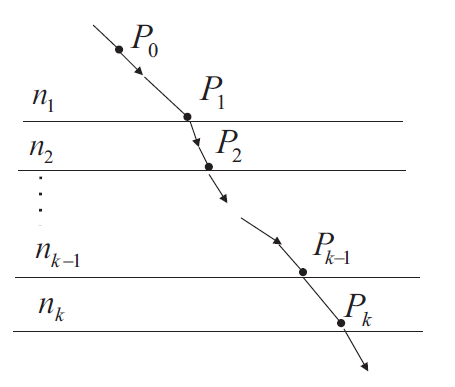
\includegraphics[scale=1]{Imagenes/Optica_Geometrica_01.png}
    \caption{Trayectoria de un rayo de luz a través de una serie de medios estratificados con diferentes
    índices de refracción.}
    \label{fig:figura_01}
\end{figure}
Entendemos por camino óptico, denotado por $CO$ a la distancia óptica expresada como la suma de los productos del índice de refracción por la distancias recorridas,
\begin{align}
CO = \overline{P_{0} \, P_{1}} n_{1} + \overline{P_{1} \, P_{2}} n_{2} + \ldots + \overline{P_{k-1} \, P_{k}} n_{k} = \nsum_{i=1}^{k} \overline{P_{i-1} \, P_{i}} n_{i}
\label{eq:ecuacion_08}
\end{align}
Cuando los estratos de los materiales cambian de punto a punto, entonces el camino óptico puede expresarse como la siguiente integral de línea:
\begin{align}
CO = \scaleint{6ex}_{\bs A}^{B} n (x, y, z) \dd{s} = \scaleint{6ex}_{\bs C} n \dd{s}
\label{eq:ecuacion_09}
\end{align}
donde $A = P_{0}$ y $B = P_{k}$, y $\dd{s}$ denota el elemento de longitud de arco sobre la curva $C$ que une los puntos extremos $A$ y $B$. Estos tipos de materiales reciben el nombre de materiales o vidrios con \textit{índice de refracción gradiente}.

\section{Dos principios fundamentales.}

En relación con las leyes básicas de la reflexión y la refracción hay dos principios fundamentales de la óptica clásica que pueden emplearse para deducir estas leyes. 

\subsection{Principio de Fermat.}

El trayecto seguido por la luz al ir de un punto $A$ a un punto $B$ en un medio material heterogéneo de índice $n(x, y, z)$ corresponde a un valor estacionario del camino óptico en relación a los caminos posibles que unen $A$ con $B$. En otras palabras, si $\dd{s}$ representa el elemento de arco de la curva $C$ que une los puntos $A$ y $B$ entonces el valor numérico dado por la integral de la ec. (\ref{eq:ecuacion_09}) es estacionario (ver esquema izquierdo en la fig. \ref{fig:figura_02}).
\begin{figure}[H]
    \centering
    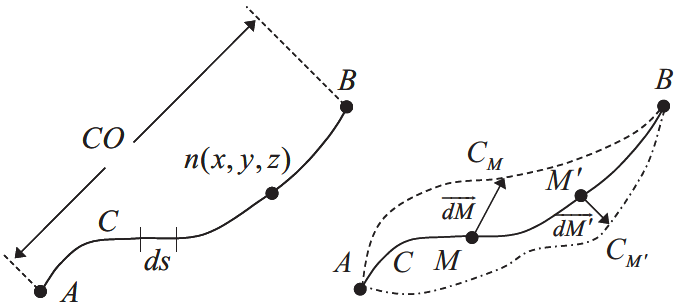
\includegraphics[scale=0.75]{Imagenes/Optica_Geometrica_02.png}
    \caption{Izquierda, curva $C$ que sigue la luz entre dos puntos $A$ y $B$ inmersos en un medio continuo heterogéneo con índice de refracción $n(x, y, z)$ para determinar el $CO$; derecha, posibles trayectorias $CM$ y $CM^{\prime}$ entre $A$ y $B$ cercanas a $C$ con valor estacionario para el $CO$.}
    \label{fig:figura_02}
\end{figure}
Para precisar el significado de este enunciado consideremos la curva $C$ como aquella que en efecto sigue la luz, i. e., un rayo al ir de $A$ a $B$. Sea $M$ un punto arbitrario en la misma curva con $M \neq A$ y $M \neq B$; los caminos vecinos a $C$ son las curvas $C_{M}$ obtenidas al desplazar en cierta dirección el punto $M$ de $C$ en una cantidad infinitesimal, denotada por $\overline{\dd{M}}$ y que igualmente comienzan en $A$ y terminan en $B$. El esquema derecho de la fig. \ref{fig:figura_02} muestra gráficamente esta situación para dos puntos intermedios distintos $M$ y $M^{\prime}$ de $C$. 

Sea $L_{AB}$ el $CO$ a lo largo de $C$ y sea $L_{AB}^{\prime}$ el $CO$ a lo largo de $C_{M}$, entonces, se dice que $L_{AB}$ es un valor estacionario si:
\begin{align*}
\abs{L_{AB}^{\prime} - L_{AB}} \leq c_{0} \, \abs{\overline{\dd{M}}}^{2}
\end{align*}
siempre que $\overline{\dd{M}} < \epsilon_{0}$ siendo $c_{0}$, $\epsilon_{0}$ constantes positivas. Es importante hacer notar que el concepto de \textit{valor estacionario} puede corresponder al caso de un valor mínimo, máximo o constante.

El principio de Fermat se puede enunciar de la siguiente manera: \enquote{De todas las trayectorias geométricamente posibles para que la luz viaje de un punto $A$ a otro punto $B$, sólo son permitidas físicamente aquellas que tienen un valor extremo (máximo, mínimo o estacionario) para el camino óptico}.

El principio de Fermat es el análogo óptico del principio de mínima acción de la mecánica. Este principio no se puede probar por medio de la óptica geométrica, pero sí con la óptica física o de ondas.

\section{Leyes de la reflexión y la refracción.}

Utilizando el principio de Fermat las leyes de la reflexión y la refracción se pueden deducir en forma muy simple, como veremos en seguida.

\subsection{Reflexión.}

La primera ley de la reflexión dice que el rayo incidente, el rayo reflejado y la normal a la superficie reflectora están en un plano común. Esta ley es una consecuencia obvia del principio de Fermat.

La segunda ley dice que la magnitud del ángulo de reflexión es igual a la magnitud del ángulo de incidencia. Consideremos la figura (\ref{fig:figura_03}, donde un rayo de luz parte del punto $P_{1} (0, y_{1})$ y llega al punto $P_{2} (x_{2}, y_{2})$ después de reflejarse en un espejo plano sobre el punto $P (x, 0)$.
\begin{figure}[H]
    \centering
    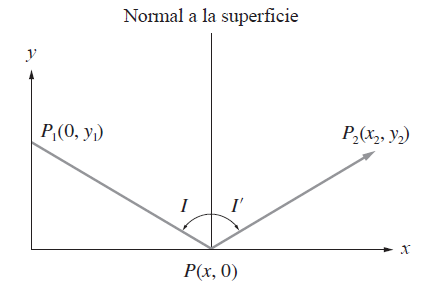
\includegraphics[scale=0.75]{Imagenes/Optica_Geometrica_03.png}
    \caption{Diagrama que ilustra la ley de reflexión, cuando el rayo sale de $P_{2}$, cuando se refleja sobre el eje x.}
    \label{fig:figura_03}
\end{figure}
Si el índice de refracción es 1.0 el camino óptico del punto $P_{1}$ al punto $P_{2}$ es:
\begin{align}
CO = n (x^{2} + y^{2})^{\frac{1}{2}} + n \left[ (x^{2} + y^{2})^{2} + y_{2}^{2} \right]^{\frac{1}{2}}
\label{eq:ecuacion_I_05}
\end{align}
Como este camino óptico tiene que ser un extremo, imponemos la condición:
\begin{align}
\dfrac{\dd{CO}}{\dd{x}} = \dfrac{n \, x}{n (x^{2} + y_{1}^{2})^{\frac{1}{2}}} - \dfrac{n \,(x_{2} - x)}{ \left[ (x^{2} - x)^{2} + y_{2}^{2}) \right]^{\frac{1}{2}}} = 0
\label{eq:ecuacion_I_06} 
\end{align}
de donde se ve que:
\begin{align}
\sin I = - \sin I^{\prime}
\label{eq:ecuacion_I_07}
\end{align}
por tanto: $I = I^{\prime}$, que es la segunda ley de la reflexión.

\subsection{Refracción.}

La primera ley de la refracción dice que el rayo incidente, el rayo refractado y la normal a la superficie refractora están en un plano común. Esta ley también es una consecuencia inmediata del principio de Fermat.
\begin{figure}[H]
\centering
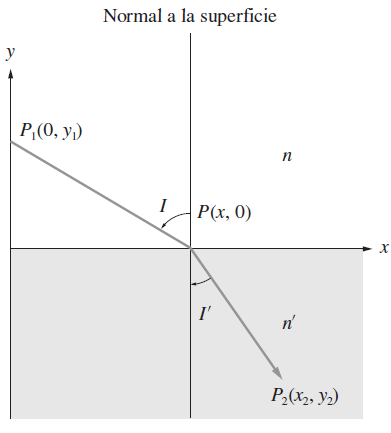
\includegraphics[scale=0.75]{Imagenes/Optica_Geometrica_04.png}
\caption{Diagrama que ilustra la ley de refracción, cuando el rayo sale de $P_{1}$ y llega a $P_{2}$, después de refractarse sobre el eje $x$.}
\label{fig:figura_04}
\end{figure}
La segunda ley, llamada también ley de Snell, se puede deducir de la figura (\ref{fig:figura_04}) donde es fácil ver que el camino óptico está dado por:
\begin{align}
CO = n (x^{2} + y^{2})^{\frac{1}{2}} + n^{\prime} \left[ (x^{2} - x)^{2} + y_{2}^{2} \right]^{\frac{1}{2}}
\label{eq:ecuacion_I_08}
\end{align}
Por el principio de Fermat debemos de imponer la condición:
\begin{align}
\dfrac{\dd{CO}}{\dd{x}} = \dfrac{n \, x}{n (x^{2} + y_{1}^{2})^{\frac{1}{2}}} - \dfrac{n^{\prime} \,(x_{2} - x)}{ \left[ (x^{2} - x)^{2} + y_{2}^{2}) \right]^{\frac{1}{2}}} = 0
\label{eq:ecuacion_I_09} 
\end{align}
de donde tenemos que:
\begin{align}
n \, \sin I = n^{\prime} \, \sin I^{\prime}
\label{eq:ecuacion_I_10}
\end{align}
que es la ley de Snell.

\subsection{Ángulo crítico.}

Consideremos, como se muestra en la figura (\ref{fig:figura_05}), muchos rayos luminosos que llegan desde todas las direcciones posibles a un agujerito muy pequeño sobre una superficie refractora.
\begin{figure}[H]
\centering
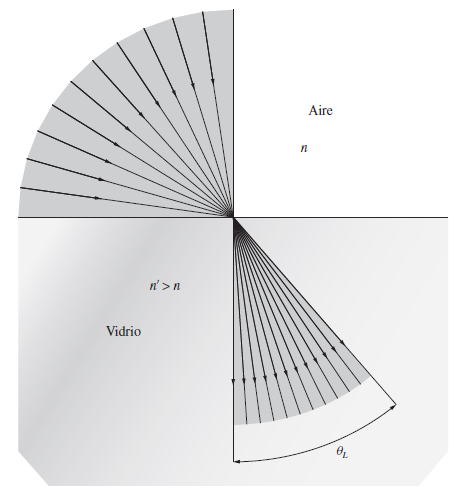
\includegraphics[scale=0.75]{Imagenes/Optica_Geometrica_05.png}
\caption{Abanico de rayos refractados con un semidiámetro angular igual al ángulo crítico, cuando los rayos entran en todas direcciones a través de una pequeña perforación.}
\label{fig:figura_05}
\end{figure}
Un rayo con un ángulo de incidencia de \ang{90} se refracta con un ángulo $\theta_{L}$ que se puede obtener de la ley de Snell:
\begin{align}
\sin \theta_{L} = \dfrac{n}{n^{\prime}}
\label{eq:ecuacion_I_19}
\end{align}
De aquí podemos observar entonces fácilmente que no existirán rayos refractados con un ángulo mayor que $\theta_{L}$. Este ángulo, llamado \textit{ángulo crítico, ángulo límite o ángulo de reflexión total}, es función únicamente del índice de refracción del material.

Un rayo que llegara a la superficie refractora desde el lado del índice de refracción mayor $n_{1}$ con un ángulo de incidencia mayor que el ángulo crítico no podrá refractarse. Este fenómeno, llamado de \textit{reflexión total interna}, es el principio de trabajo de muchos prismas.

\section{Trazo de rayos en una superficie esférica.}

La superficie esférica refractora es la más común y la más útil en óptica, después de la plana. En una superficie refractora como la que se muestra en la figura (\ref{fig:figura_10}) podemos definir los siguientes parámetros:
\begin{enumerate}[label=\alph*)]
\item \textit{Centro de curvatura}: es el centro de una esfera imaginaria que contiene a la superficie refractora.
\item \textit{Radio de curvatura}: es la distancia de la superficie refractora al centro de curvatura.
\item \textit{Vértice}: es un punto sobre la superficie refractora, en el centro de su abertura libre. Esta abertura se supone de forma circular.
\item \textit{Eje óptico}: es una línea recta imaginaria que pasa por el vértice y el centro de curvatura.
\end{enumerate}
\begin{figure}[H]
    \centering
    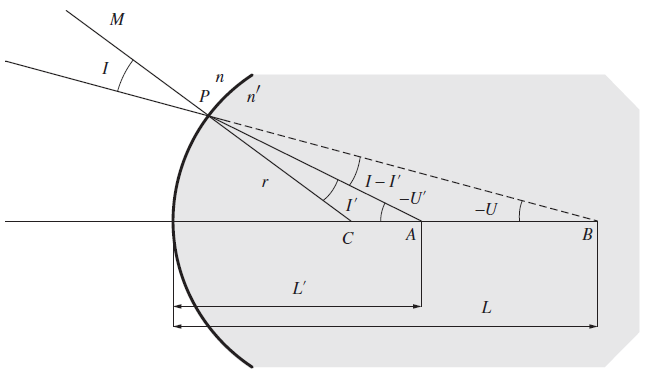
\includegraphics[scale=0.75]{Imagenes/Optica_Geometrica_06.png}
    \caption{Refracción de un rayo meridional en una superficie que separa dos medios.}
    \label{fig:figura_10}
\end{figure}
A una superficie esférica refractora pueden llegar rayos luminosos con muy diversas orientaciones. Según su dirección, los rayos que inciden en una superficie esférica se pueden clasificar en los siguientes tipos:
\begin{enumerate}
\item \textit{Rayo meridional}: es cualquier rayo que junto con el eje óptico definen un plano al que llamamos \underline{meridional}. En este caso la normal a la superficie y el rayo refractado están también en el plano meridional.
\item \textit{Rayo oblicuo}: es cualquier rayo que no sea meridional. En este caso el rayo ni tiene un punto común con el eje óptico ni es paralelo a él.
\item \textit{Rayo paraxial}: es un rayo meridional cuyo ángulo con respecto al eje óptico es muy pequeño (paraxial significa cerca del eje).
\end{enumerate}
En conexión con la teoría de aberraciones, los rayos tangenciales y los sagitales, que se pueden ilustrar mediante la figura (\ref{fig:figura_11}).
\begin{figure}[H]
    \centering
    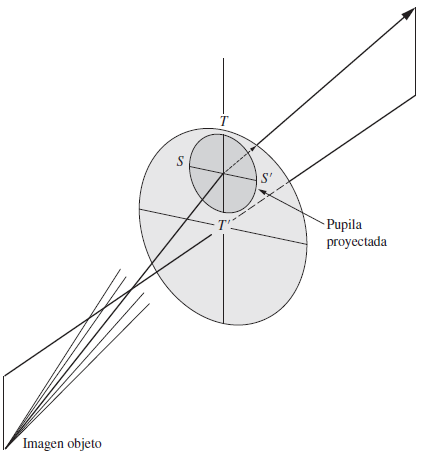
\includegraphics[scale=0.75]{Imagenes/Optica_Geometrica_07.png}
    \caption{Ilustración de los conceptos de rayos sagitales y rayos tangenciales.}
    \label{fig:figura_11}
\end{figure}
Supongamos un objeto real o virtual fuera del eje óptico, frente a una superficie óptica esférica. Los rayos luminosos que iluminan esta superficie parten todos de este objeto y llegan todos a la superficie, pasando por una abertura circular descentrada. Esta abertura es una imagen de la abertura circular a la entrada del sistema óptico y le llamaremos pupila proyectada. De todos estos rayos, a aquellos que pasan sobre la línea $T T^{\prime}$ les llamaremos \textit{rayos tangenciales}. A aquellos que pasan sobre la línea $S S^{\prime}$ les llamaremos \textit{rayos sagitales}. Al rayo que pasa por el centro de la pupila proyectada le llamamos \textit{rayo principal}. Los rayos tangenciales son un caso particular de rayos meridionales. El plano meridional se llamaría en este caso plano tangencial. Los rayos sagitales son un caso particular de rayos oblicuos y están contenidos en un plano llamado plano sagital, perpendicular al tangencial. Además se han definido los rayos parabasales, en analogía con los rayos paraxiales, que son todos aquellos que vienen del objeto fuera de eje, viajando muy cerca del rayo principal. Parabasal significa cerca de la base.

La figura (\ref{fig:figura_10}) muestra una superficie esférica refractora y un rayo meridional que incide en el punto $P$. La normal a la superficie en el punto $P$ es $M$ y el centro de curvatura es $C$.

Por definición, todos los parámetros $r, L, L^{\prime}, I, I^{\prime}$, excepto $U$ y $U^{\prime}$, son positivos en la figura (\ref{fig:figura_10}). De hecho, el radio de curvatura $r$ es positivo si el centro de curvatura está a la derecha del vértice y negativo si está a la izquierda de éste; las distancias $L$ y $L^{\prime}$ son positivas si sus respectivos cruces $A$ o $B$ están a la derecha del vértice y negativas si están a la izquierda; los ángulos $U$ y $U^{\prime}$ tienen el mismo signo de sus pendientes; los ángulos $I$ y $I^{\prime}$ son positivos si sus pendientes son mayores, considerando su signo, que la pendiente de la normal $M$ y negativos en caso contrario, y los ángulos $I$ y $I_{1}$ tienen el mismo signo en una refracción y signo contrario en una reflexión.

Aplicando la ley trigonométrica del seno al triángulo $PCB$:
\begin{align}
\dfrac{\sin I}{L - r} = - \dfrac{\sin U}{r}
\label{eq:ecuacion_I_20}
\end{align}
y aplicando la misma ley al triángulo $PCA$:
\begin{align}
\dfrac{\sin I^{\prime}}{L^{\prime} - r} = - \dfrac{\sin U^{\prime}}{r}
\label{eq:ecuacion_I_21}
\end{align}
aplicando ahora una bien conocida relación entre los ángulos de un triángulo al $PAB$:
\begin{align}
U - I = U^{\prime} - I^{\prime}
\label{eq:ecuacion_I_22}
\end{align}
La última relación que necesitamos es la ley de Snell:
\begin{align}
n \, \sin I = n^{\prime} \, I^{\prime}
\label{eq:ecuacion_I_23}
\end{align}
En estas cuatro relaciones los parámetros $r, n y n^{\prime}$ son en general fijos y conocidos, y las cantidades $L, L^{\prime}, I, I^{\prime}, U, U^{\prime}$ son variables. Como tenemos cuatro ecuaciones, todas las variables pueden ser calculadas si dos cualquiera de los tres parámetros $L, I, U$, para el rayo incidente son especificados.

Un rayo paraxial es un rayo meridional cuyos ángulos $I$ y $U$ son tan pequeños que $\sin I$ y $\sin U$ pueden ser remplazados sin sacrificar mucha precisión por los valores de $I$ y de $U$ expresados en radianes. Llamamos \textit{óptica de primer orden} a la óptica geométrica que considera sólo rayos paraxiales. 

Las ecuaciones básicas de la óptica de primer orden se mantienen haciendo los siguientes remplazos en las ecuaciones (\ref{eq:ecuacion_I_20}) a (\ref{eq:ecuacion_I_23}):
\begin{align}
\begin{aligned}
\sin I &\Rightarrow i \\
\sin I^{\prime} &\Rightarrow i^{\prime} \\
\sin U &\Rightarrow u \\
\sin U^{\prime} &\Rightarrow u^{\prime} \\
L &\Rightarrow l \\
L^{\prime} &\Rightarrow l^{\prime}
\end{aligned}
\label{eq:ecuacion_I_24}
\end{align}
se obtiene así:
\begin{eqnarray}
\dfrac{i}{l - r} &=& - \dfrac{u}{r} \label{eq:ecuacion_I_25} \\ [0.5em]
\dfrac{i^{\prime}}{l^{\prime} - r} &=& - \dfrac{u^{\prime}}{r} \label{eq:ecuacion_I_26} \\ [0.5em]
u - i &=& u^{\prime} - i^{\prime} \label{eq:ecuacion_I_27} \\ [0.5em]
n \, i &=& n^{\prime} \, i^{\prime} \label{eq:ecuacion_I_28}
\end{eqnarray}
Las variables $L$ y $L^{\prime}$ se han sustituido por $l$ y $l^{\prime}$ para tener presente que los valores obtenidos con estas ecuaciones son sólo aproximaciones de primer orden. La mayor parte de las propiedades de las lentes y sistemas ópticos se pueden obtener con bastante precisión usando óptica de primer orden, con la única excepción de las aberraciones monocromáticas.

\section{Fórmula de Gauss.}

Esta fórmula representa uno de los resultados más importantes de la teoría de primer orden y se puede derivar directamente de las ecuaciones (\ref{eq:ecuacion_I_25}) a (\ref{eq:ecuacion_I_28}). Deduciremos esta fórmula a partir de las ecuaciones exactas y las aproximaciones de primer orden se harán al final. De la ecuación (\ref{eq:ecuacion_I_20}) podemos obtener:
\begin{align}
\dfrac{L}{r} = - \dfrac{\sin I}{\sin U} + 1 = \dfrac{\sin U - \sin I}{\sin U}
\label{eq:ecuacion_I_29}
\end{align}
de aquí podemos ver que:
\begin{align}
\dfrac{r}{L} = 1 - \dfrac{\sin I}{\sin I - \sin U}
\label{eq:ecuacion_I_30}
\end{align}
y luego multiplicando ambos lados por $n/r$:
\begin{align}
\dfrac{n}{L} = \dfrac{n}{r} - \dfrac{n}{r} \dfrac{\sin I}{\sin I - \sin U}
\label{eq:ecuacion_I_31}
\end{align}
de manera similar, usando la ec. (\ref{eq:ecuacion_I_21}):
\begin{align}
\dfrac{n^{\prime}}{L^{\prime}} = \dfrac{n^{\prime}}{r} - \dfrac{n^{\prime}}{r} \dfrac{\sin I^{\prime}}{\sin I^{\prime} - \sin U^{\prime}}
\label{eq:ecuacion_I_32}
\end{align}
Si se resta ahora la ec. (\ref{eq:ecuacion_I_31}) de la ec. (\ref{eq:ecuacion_I_32}) miembro a miembro, se obtiene:
\begin{align}
\dfrac{n^{\prime}}{L^{\prime}} - \dfrac{n}{L} = \dfrac{n^{\prime} - n}{r} + \dfrac{n \, \sin I}{r} \left[ \dfrac{1}{\sin I - \sin U} - \dfrac{1}{\sin I^{\prime} - \sin U^{\prime}} \right]
\label{eq:ecuacion_I_33}
\end{align}
si usamos aquí las aproximaciones para rayos paraxiales (primer orden) obtenemos finalmente la \textit{fórmula de Gauss}:
\begin{align}
\dfrac{n^{\prime}}{l^{\prime}} - \dfrac{n}{l} = \dfrac{n^{\prime} - n}{r}
\label{eq:ecuacion_I_34}
\end{align}
Esta fórmula nos da la distancia $l^{\prime}$ de la superficie refractora a la imagen, conocida la distancia $l$ de la superficie al objeto. Dada la distancia $l^{\prime}$, con independencia del ángulo de incidencia. De aquí podemos concluir que, dentro de los límites de la óptica de primer orden, la imagen de un objeto puntual es también puntual.

Si la altura del rayo paraxial meridional en el cruce de la superficie óptica es $y$, podemos escribir:
\begin{align}
u = - \dfrac{y}{l} \hspace{1cm} \text{y} \hspace{1cm} u^{\prime} = - \dfrac{y}{l^{\prime}}
\label{eq:ecuacion_I_35}
\end{align}
y para encontrar el valor de $y$ en la siguiente superficie tenemos:
\begin{align}
y_{+1} = y + t \, u^{\prime}
\label{eq:ecuacion_I_36}
\end{align}
De estas definiciones podemos expresar la ecuación de Gauss en forma alternativa como:
\begin{align}
- n^{\prime} \, u^{\prime} + n \, u = (n^{\prime} - n) \, c \, y
\label{eq:ecuacion_I_37} 
\end{align}
donde la curvatura $c = 1/r$.

\section{Formación de imágenes.}

Una superficie refractora, una lente o un sistema de lentes, al formar una imagen de un objeto establece una correspondencia uno a uno entre puntos luminosos del objeto y puntos de la imagen. La función del sistema formador de imágenes es refractar (o reflejar) la luz proveniente de un punto en el objeto y enviarla a un solo punto en la imagen, como se muestra en la figura (\ref{fig:figura_12}).
\begin{figure}[H]
    \centering
    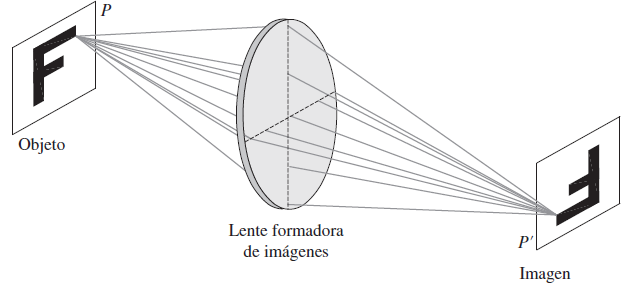
\includegraphics[scale=0.75]{Imagenes/Optica_Geometrica_08.png}
    \caption{Diagrama que ilustra el mecanismo de la formación de imágenes con una lente convergente.}
    \label{fig:figura_12}
\end{figure}
El objeto cuya imagen se va a formar puede ser de cualquiera de los siguientes dos tipos:
\begin{enumerate}[label=\alph*)]
\item \textit{Objeto real}: el objeto es real cuando la distancia $L$ para la primera superficie refractora es negativa, es decir cuando el objeto está a la izquierda del sistema óptico, como se muestra en las figuras (\ref{fig:figura_13})  y (\ref{fig:figura_15}). El objeto es real cuando a la izquierda de la lente está el objeto físico mismo o una imagen formada ahí por otro sistema óptico.
\item \textit{Objeto virtual}: consideremos otro sistema colocado entre el sistema óptico de la figura (\ref{fig:figura_12}) y su imagen. Este otro sistema cambiará la posición y el tamaño y quizá la orientación de la imagen. Por simple convención se dice en este caso que la imagen formada por el primer sistema es el objeto del cual forma una nueva imagen el segundo sistema. Como el objeto del segundo sistema está a la derecha de él, se plantea que es un objeto virtual. En este caso $L$ es positiva, como se puede observar en las figuras (\ref{fig:figura_14}) y (\ref{fig:figura_16}).
\end{enumerate}
\begin{figure}[H]
    \centering
    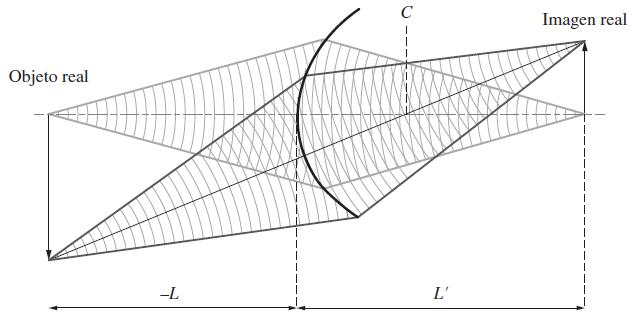
\includegraphics[scale=0.75]{Imagenes/Optica_Geometrica_09.png}
    \caption{Formación de la imagen real de un objeto real, por medio de una superficie esférica con la convexidad hacia el objeto. El índice de refracción es mayor del lado de la imagen.}
    \label{fig:figura_13}
\end{figure}
\begin{figure}[H]
    \centering
    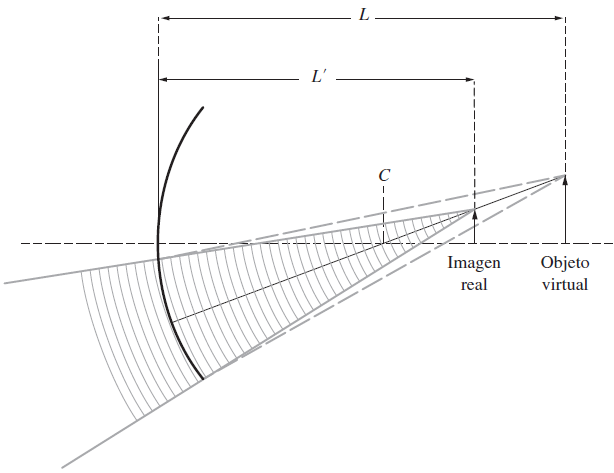
\includegraphics[scale=0.75]{Imagenes/Optica_Geometrica_10.png}
    \caption{Formación de la imagen real de un objeto virtual, por medio de una superficie esférica con la convexidad hacia el objeto. El índice de refracción es mayor del lado de la imagen.}
    \label{fig:figura_14}
\end{figure}
Al igual que el objeto, la imagen también puede ser real o virtual, como veremos en seguida:
\begin{enumerate}[label=\roman*)]
\item \textit{Imagen real}: una imagen real se puede observar de dos maneras: colocando una pantalla en el lugar donde se forma la imagen, u observándola directamente con el ojo desde una distancia grande a la derecha de donde la imagen se ha formado. En este caso la distancia $L$ es siempre positiva, como se ve en las figuras (\ref{fig:figura_13}) y (\ref{fig:figura_14}).
\item \textit{Imagen virtual}: los rayos que parten de un punto del objeto pueden no converger sino divergir después de pasar por el sistema óptico y, por lo tanto, no formar ninguna imagen real. Sin embargo, los rayos tendrán un punto aparente de convergencia, formando así una imagen virtual. Este tipo de imágenes pueden observarse con el ojo, pero no se pueden formar sobre una pantalla. En este caso la distancia $L$ es siempre negativa, como se ve en las figuras (\ref{fig:figura_15}) y (\ref{fig:figura_16}).
\end{enumerate}
\begin{figure}[H]
    \centering
    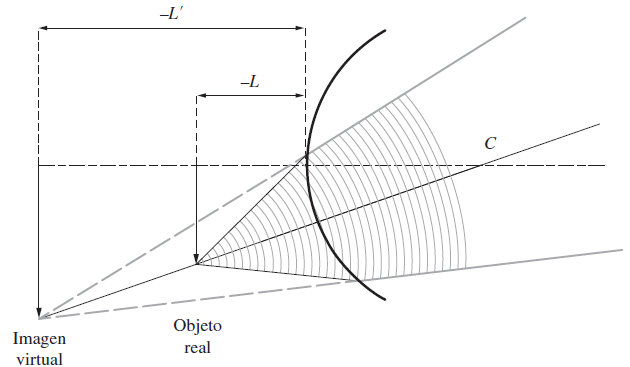
\includegraphics[scale=0.75]{Imagenes/Optica_Geometrica_11.png}
    \caption{Formación de la imagen virtual de un objeto real por medio de una superficie esférica con la convexidad hacia el objeto. El índice de refracción es mayor del lado de la imagen.}
    \label{fig:figura_15}
\end{figure}
\begin{figure}[H]
    \centering
    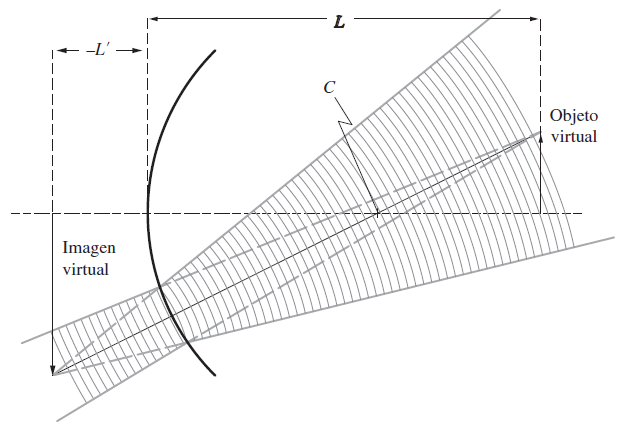
\includegraphics[scale=0.75]{Imagenes/Optica_Geometrica_12.png}
    \caption{Formación de la imagen virtual de un objeto virtual, por medio de una superficie esférica con la convexidad hacia el objeto. El índice de refracción es mayor del lado de la imagen.}
    \label{fig:figura_16}
\end{figure}

\section{Teoremas del seno y de Lagrange.}

El teorema óptico del seno establece una relación entre el tamaño de la imagen y el g rado de convergencia o divergencia de los rayos en el plano de la imagen. Este teorema lo deduciremos aquí usando la figura (\ref{fig:figura_17}), donde todos los parámetros ahí indicados son positivos.
\begin{figure}[H]
\centering
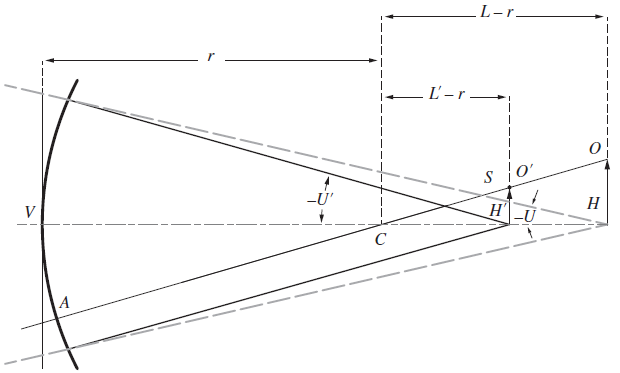
\includegraphics[scale=0.65]{Imagenes/Optica_Geometrica_13.png}
\caption{Diagrama para deducir la ley del seno.}
\label{fig:figura_17}
\end{figure}
Si suponemos que el campo es muy pequeño, de tal forma que $H$ sea mucho menor que $L$, podemos observar que:
\begin{align}
\dfrac{H^{\prime}}{H} = \dfrac{L^{\prime} - r}{L - r}
\label{eq:ecuacion_I_44}
\end{align}
Utilizando ahora las ecuaciones (\ref{eq:ecuacion_I_20}) y (\ref{eq:ecuacion_I_20}) podemos constatar que:
\begin{align}
n \, H \, \sin U = n^{\prime} \, H^{\prime} \, \sin U^{\prime}
\label{eq:ecuacion_I_45}
\end{align}
Éste es el \textit{teorema óptico del seno}. Si consideramos un par de rayos sagitales simétricamente colocados respecto al plano meridional podemos fácilmente concluir que después de refractarse en la superficie óptica se cruzarán en el plano meridional. Además, este punto de cruce está sobre el eje principal, que es la línea $AO$.

Este punto de cruce es la imagen sagital. Después de estudiar con detalle las aberraciones se puede concluir que este teorema es exacto sólo para campos pequeños, si la abertura es relativamente pequeña (rayos paraxiales) y si los rayos considerados son sagitales.

El triple producto $n \, H \, \sin U$ se dice que es un invariante óptico porque en cualquier sistema óptico formado con superficies refractoras y/o reflectoras centradas su magnitud es la misma antes y después de cualquier superficie. Se dice que el sistema óptico está formado de superficies centradas cuando todos sus centros de curvatura están sobre una recta común llamada eje óptico.

La aproximación paraxial de este teorema se conoce con el nombre de \textit{teorema de Lagrange} y se escribe:
\begin{align}
h \, n \, u = h^{\prime} \, n^{\prime} \, u^{\prime}
\label{eq:ecuacion_I_46}
\end{align}
La principal aplicación de este teorema es para saber la amplificación de un sistema óptico si sabemos su poder de convergencia y viceversa. Es la base de la definición de distancia focal efectiva y una herramienta sumamente útil para el análisis de sistemas ópticos.

\section{Amplificación lateral y longitudinal.}

La amplificación lateral de un sistema óptico está definida como:
\begin{align}
m = \dfrac{H^{\prime}}{H}
\label{eq:ecuacion_I_47}
\end{align}
donde $H$ es la altura del objeto y $H^{\prime}$ la altura de la imagen. Usando el teorema óptico del seno podemos ver que esta amplificación es:
\begin{align}
m = \dfrac{H^{\prime}}{H} = \dfrac{n \, \sin U}{n^{\prime} \, \sin U^{\prime}} 
\label{eq:ecuacion_I_48}
\end{align}
De esta expresión podemos concluir que un sistema óptico tendrá una amplificación íntimamente ligada a su grado de convergencia y que no es posible modificar una sin modificar la otra, a menos que también cambie el cociente $n/n^{\prime}$. La amplificación lateral en su aproximación paraxial es:
\begin{align}
m = \dfrac{h^{\prime}}{h} = \dfrac{n \, u}{n^{\prime} \, u^{\prime}} 
\label{eq:ecuacion_I_49}
\end{align}

\section{Materiales ópticos.}

Los materiales utilizados en la fabricación de componentes ópticos son muy diversos y con propiedades físicas que dependen de la aplicación. A continuación se describirán brevemente los principales, citando sus aplicaciones más comunes así como sus propiedades más relevantes:
\begin{enumerate}[label=\alph*)]
\item \textit{Vidrio óptico}: el vidrio óptico, como todos los vidrios, tiene como componente básico el dióxido de silicio (SiO2) o cuarzo, el cual se extrae de algunas arenas. Las principales diferencias que hay entre el vidrio óptico y otros tipos ordinarios de vidrio son su alta homogeneidad y su transparencia. La homogeneidad se logra por medio de procesos de fabricación adecuados que mezclen bien las sustancias mientras están calientes, esto es, en estado fluido. La transparencia se obtiene utilizando arenas y productos químicos de alta pureza. El color verde del vidrio que se usa en las ventanas, por ejemplo, se debe a la presencia del óxido de fierro en las arenas.

El índice de refracción es la principal constante óptica que caracteriza un vidrio óptico. Como se ha visto antes, este índice es función de la longitud de onda, pues mientras más alta sea la frecuencia, o lo que es lo mismo, más corta la longitud de onda, mayor será el índice de refracción. A fin de tomar en cuenta esta dispersión cromática del índice de refracción, se ha definido otra constante $V$, llamada número de Abbe, que se define como:
\begin{align}
V = \dfrac{n_{D} - 1}{n_{F} - n_{C}}
\label{eq:ecuacion_I_59}
\end{align}
donde los subíndices $D, F$ y $C$ representan los colores amarillo, azul y rojo, respectivamente. De esta manera un vidrio se puede caracterizar por medio de dos constantes, $n_{D}$ y $V$, cuyos valores se pueden determinar al fabricar el vidrio, esto es, mediante el control de ciertos aditivos, como el óxido de plomo y el bario.

Estas letras corresponden a las líneas del espectro solar descubiertas por Fraunhofer, de acuerdo con la siguiente tabla:
\begin{table}[H]
    \centering
    \begin{tabular}{c | c | c | c}
        Línea espectral & Longitud de onda en nm & Elemento & Color \\ \hline
        h & \num{404.66} & Hg & Ultravioleta \\ \hline
        g & \num{435.84} & Hg & Azul \\ \hline
        F & \num{486.13} & H & Azul \\ \hline
        d & \num{587.56} & He & Amarillo \\ \hline
        D & \num{589.29} & Na & Amarillo \\ \hline
        C & \num{656.27} & H & Rojo \\ \hline
    \end{tabular}
\end{table}
\item \textit{Vidrios con baja expansión térmica}: en la fabricación de espejos ópticos con capa reflectora frontal no es importante ni la transparencia ni la homogeneidad del vidrio, sino su bajo coeficiente de expansión térmica, a fin de evitar que se deforme con los cambios de la temperatura ambiente.
\item \textit{Plásticos}: los plásticos también encuentran una gran aplicación en la fabricación
de componentes ópticos de bajo costo. Mediante los procesos de moldeo o prensado es posible fabricar rápidamente y con un costo razonable lentes esféricas.

El problema de las lentes de plástico es que ni la transparencia, ni la homogeneidad, ni la calidad de la superficie se pueden igualar a las de las lentes de vidrio. Además, la resistencia a la abrasión y a las altas temperaturas también es menor que las de vidrio.
\item \textit{Materiales para uso en el infrarrojo y el ultravioleta}: los vidrios y plásticos son transparentes en la región visible del espectro óptico, pero no en el infrarrojo ni en el ultravioleta. De los vidrios ópticos comunes, el que tiene la región espectral transparente más amplia es el N-BK7, que va desde \num{350} hasta \SI{2}{\micro\meter}. Cuando es necesaria una buena transparencia en el infrarrojo se usan los materiales especiales. Entre ellos se encuentran el silicio fundido de grado UV que comienza a ser transparente desde los \SI{300}{\nano\meter}, ascendiendo hasta \SI{4}{\micro\meter} y finalmente cortar alrededor de \SI{3}{\micro\meter}. Existen varios materiales, principalmente cristales, con muy buenas características en el infrarrojo y en el ultravioleta, pero generalmente son muy caros.
\end{enumerate}
\end{document}